\chapter{Technical Design}
\label{chap:technical}

\section{Project Scope}
By design this project aims to create a generalisable robot learning algorithm which will have applications in multiple problem scenarios. The generalisability comes from the ability to provide a robot with whatever demonstrations are relevant to solving the desired task, without requiring any changes to the core system. However, in the interest of keeping this project focused we choose to implement and analyse specifically an agent for generalised object manipulation tasks focused around grasping and moving simple objects. 
\\

\subsection{Environment specifics}
\label{subsec:pybullet-specifics}
For this project we conduct the experiments in a real time physics engine, called \socalled{PyBullet} \cite{pybullet}, available as an open source python package. As such the algorithms presented in this paper will be implemented in Python and the experimental results and evaluation will be conducted in this simulation space.\\
The specific robot arm used throughout this project is a simulation of the \socalled{Franka Panda robot arm}, which comes built in with PyBullet. This arm can be seen in \reffig{fig:arm-normal}.

\begin{figure}[h]
    \centering
    \begin{subfigure}[b]{0.45\textwidth}
        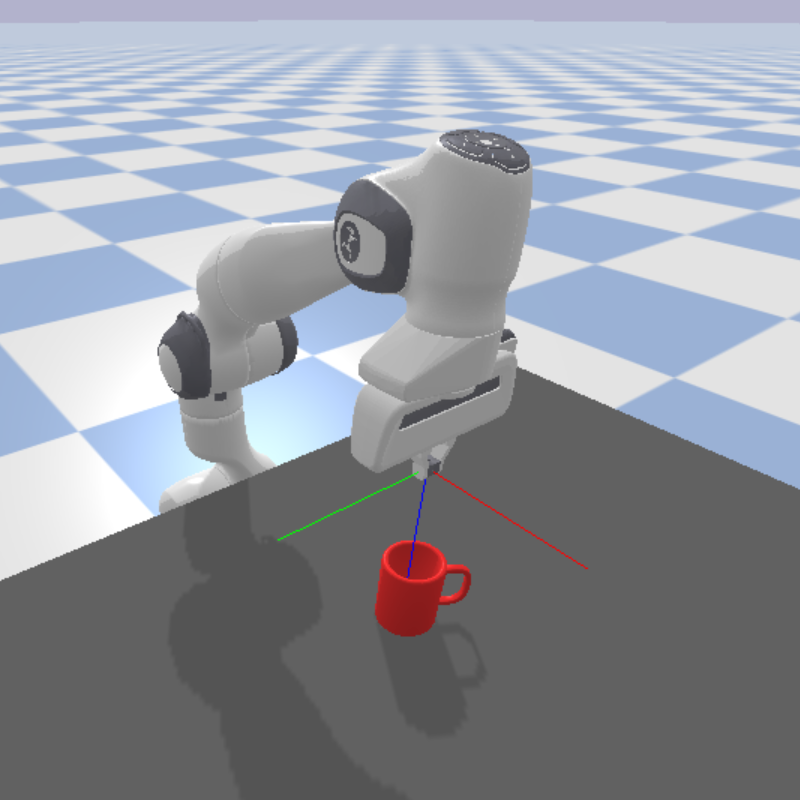
\includegraphics[width=\textwidth]{figures/robot-arm.png}
        \caption{Normal view}
        \label{fig:arm-normal}
    \end{subfigure}
    \hfill
    \begin{subfigure}[b]{0.45\textwidth}
        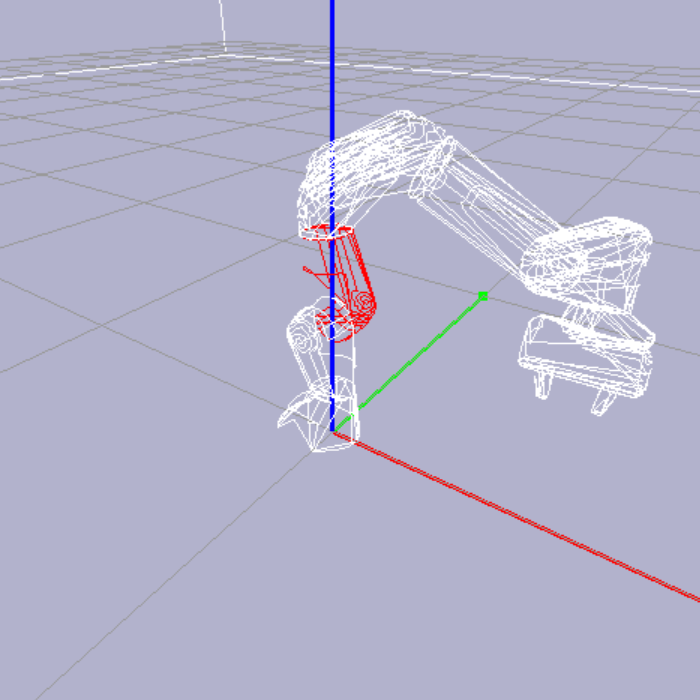
\includegraphics[width=\textwidth]{figures/robot-arm-wireframe.png}
        \caption{Wire-frame view}
        \label{fig:arm-wire}
    \end{subfigure}
    \caption{Franka panda robot arm in PyBullet simulation}
    \label{fig:robot-arm}
\end{figure}

This simulation and arm have a number of intricacies which posed a steep learning curve near the start of this project. This subsection highlights a few of these. The first major hurdle was with the accuracy of the inverse kinematics system built into Pybullet. The initial inaccuracies were not a bug in the simulation, but a misunderstanding of the signature of some of the functions.
The Franka panda robot arm has 12 individual joints. However, upon closer inspection it becomes apparent that 3 of these joints are not actuated and are fixed in place relative to the previous joint. As such the arm only has 9 degrees of freedom, while reporting all 12 joints. This issue is only apparent when using inverse kinematics to calculate the joint angles to reach a desired end effector position, since this function returns a list of length equal to the degrees of freedom of the arm. This means we get a list of 9 angles instead of 12. The function to control the arm motors, \verb|pybullet.setJointMotorControlArray()| expects one angle for every joint. As such if we pass the list of joint angles directly, we end up trying to move some of the fixed joints, while leaving the top 3 joints unspecified, resulting in not moving them. While this is not difficult to fix, there are numerous inconsistencies in the signature of different functions, which are not clearly documented. Each of these issues slowing down development while it is debugged.\\

Another point of note specific to the simulation is how cameras are implemented. The camera's in Pybullet do not use the standard intrinsic and extrinsic matrix to convert world coordinate to pixel coordinates in the image. Pybullet instead uses a projection matrix and view matrix respectively. These broadly serve the same purpose with the view matrix capturing the position and orientation of the camera and the projection matrix capturing the specifics for how points are projected onto the 2d image. The most notable difference is that the projection and view matricies are $4\times4$ instead of $3\times3$, since they consider homogeneous coordinate points. In this paper we will refer to the projection and view matrix as this is what our simulation uses. However, one could easily use a system which instead requires an intrinsic and extrinsic matrix instead.

%TODO put this somewhere
 In PyBullet, orientations are represented using quaternions, \cite{quaternions}\cite{orientations} an explanation of which is provided in \refsec{sec:rotations}. Despite adding a fourth dimension, quaternions provide a big advantage over the alternative of Euler angles. This being that quaternions do not suffer from \socalled{gimbal lock}. %TODO: cite gimbal lock

\subsection{Collecting demonstrations}
In order to generate the trajectories needed for the imitation learning system, a utility program is created to streamline the collection of demonstrations. This program generates trajectories by recording key frame poses throughout the demonstration. The demonstration can be copied by matching each of these key frame poses, with interpolation poses between them.
This program allows for the user to control and move the end effector position and orientation in Cartesian world coordinates. Once the arm is positioned in the correct pose, the user can save the current pose as a key frame of the trajectory. From here they can move the arm again and save the next key frame. If a mistake is made, the user can revert the robot arm to the last saved key frame.\\
The trajectory is stored as a list of end effector poses, the reason for which will be discussed in \refsec{sec:trajectories}.

The program is written to interface with a video game controller, so that the user can control the robot using an analogue input method such as the joysticks. This makes the program slightly more user friendly, as moving the joystick only slightly will move the joint very slowly and so allows for finer control.\\
In addition to controlling the robot, the program allows for camera rotation and zooming to better see the full robot pose, and can also enable a wire-frame view, visible in Figure \ref{fig:arm-wire}.
%TODO proof read and maybe flesh this out a little more
%TODO get new figures in table environment without joint colour coding


\section{Encoding the problem}
\label{sec:trajectories}
In this paper we plan to build upon existing ideas in the field while reducing the barrier to entry formed by using extremely resource intensive AI models. We intend to provide the robot with an example trajectory which successfully accomplishes the skill, in addition to some further context which allows the robot to generalise this trajectory to different environments. The nature of this context will be discussed further in \refsec{sec:dinobot}.\\

Let us formalise the concept of a demonstration trajectory, as this will be key in understanding how we can extract useful information from the environment it was presented in, into other unseen environments. Firstly we decompose the state of the system at time t as the current state of the robot and the state of the environment.
$$s_t = (s^{(r)}_t, s^{(e)}_t)$$

\subsection{Robot state}
We have a number of options for how to represent the state of the robot. The most expressive approach is to record the angle of every joint of the robot. This uniquely defines an exact pose of the robot.
\\
Another option to encode the robot's state is to use the end effector position and orientation. This option is appealing since for the purposes of performing manipulation tasks, the end effector pose is our main concern. We likely do not care about how the robot achieves this end effector pose, so long as it does. For this reason storing only the end effector pose at each time step, and dynamically computing the joint angles to achieve this using inverse kinematics, appears to be a desirable choice.\\

However it is worth considering that in this case an end effector pose does not uniquely define the entire robot pose. This is because the end effector pose has 3 degrees of freedom for the position and 3 for the orientation (4 quaternion components however the sum of squares must equal 1, tying down the 4th value once 3 are already chosen). In contrast the robot used in this project has 9 degrees of freedom, as discussed in \refsubsec{subsec:pybullet-specifics}. This means that the inverse kinematics system of equations is underdetermined since we have in essence 6 constraints but 9 unknowns to satisfy them with. As such, the inverse kinematics has infinitely many solutions. What this means for us is that the end effector pose does not uniquely define an entire robot pose. There are in theory infinitely many robot poses which would result in the end effector reaching the position and orientation we wanted it to.\\

\reffig{fig:underdetermined} demonstrates an analogous instance in 2 dimensions for easier viewing. In this system the target position is an (x,y) position and the orientation can be defined by a single angle. This means we have 3 degrees of freedom. Therefore, a robot arm with 4 or more controllable joints would create an underdetermined system. \reffig{fig:underdetermined} showcases just 3 possible solutions, but one can imagine how infinitely many may exist. One can also extrapolate this idea into 3 dimensions.

\begin{figure}[h]
    \centering
    \begin{subfigure}[b]{0.3\textwidth}
        \includegraphics[width=\textwidth]{example-image-a.png}
    \end{subfigure}
    \hfill
    \begin{subfigure}[b]{0.3\textwidth}
        \includegraphics[width=\textwidth]{example-image-b.png}
    \end{subfigure}
    \hfill
    \begin{subfigure}[b]{0.3\textwidth}
        \includegraphics[width=\textwidth]{example-image-c.png}
    \end{subfigure}
    \caption{An underdetermined inverse kinematics system has multiple solutions}
    \label{fig:underdetermined}
\end{figure}

While this initially seems like a big problem, for our purposes we truly do only care that the end effector is in the position and orientation we want. Any of the satisfying robot poses will do. Working with the end effector pose directly also simplifies a lot of our work later on. We will see in \refsubsec{subsec:alignment} that a lot of our calculations will involve the end effector pose. While we could compute this using forward kinematics if the demonstration instead stored joint angles, this would be an unnecessary extra step for no real benefit to the accuracy of the system. A way to use the underdetermined nature of the system to our advantage is explored further in \refappendix{apx:null-space}.\\

We may optionally decide to also include velocity information in addition to positional information. This would allow us to specify that the robot should have an exact position, but also describe how it should move in the next time step. While this may be useful for very specific tasks like throwing an object to an exact target; for the majority of tasks, velocity information is simply not necessary when we have the position for the next key frame already defined. If we were to save a key frame every time step, then the velocity information would be completely redundant, with velocity being directly computable as the displacement between the two key frames divided by the time step. In practice, for usability, we opt to not do this and only record key frames when deemed necessary by the user during the demonstration. While this does mean velocity information is not directly knowable, we decide that velocity information is not necessary for the simple tasks we are experimenting with in this paper.\\

One final thing to consider with how to represent the robot state is the gripper of the end effector. We decided to use inverse kinematics and just define the position and orientation of the end effector. However, the gripper arms are attached to the end effector. Moving the gripper arms will not affect the pose of the end effector. This means that the inverse kinematics solution will still be a valid solution whatever position the gripper arms are in. Therefore, we need to add some information to our state which uniquely decides where the gripper arms are. We could use the angle of each gripper arm, however it is unlikely we would want the grippers at different angles, so we can simplify to a single angle which we mirror for both grippers. However, we can simplify even further. We do not anticipate a situation where the gripper would need to be in an intermediate half closed state. We either want the gripper fully closed, applying a constant pressure to the item it is holding, so that the item does not fall out of its grasp, or we want the gripper fully open, so that it can drop the item it is holding. As such we can see that a single boolean value is sufficient to define the gripper state in our situation.
$$g \in \{0,1\}$$

With these decisions in place we can define the robots state as an 8 vector, containing the position and orientation of the end effector, along with the gripper state. 
$$s^{(r)} = [x_{eef}, y_{eef}, z_{eef}, a_{eef}, b_{eef}, c_{eef}, d_{eef}, g]$$

\subsection{Environment State}
We define the state of objects similarly to how we defined the end effector pose storing the 3D position and orientation of the object within the scene. Objects do not have an associated gripper, so an objects state is a 7 vector. The state of the whole environment is just the collection of all the object states within the scene.
$$s^{(e)} = \{[x_o, y_o, z_o, a_o, b_o, c_o, d_o]\}_{o=1}^O$$

We note that without a perfect model of the environment, the environment's state is not fully observable. In implementation we will not be able to capture the full environment state and instead choose to represent it differently entirely. For example capturing the environment state as an image of the scene using methods similar to those employed by P. Vitiello, K. Dreczkowski, and E. Johns \cite{one-shot-pose-estimate}. For now we will continue in the purely theoretical sense, where the environment state can be fully observed.\\

\subsection{Trajectories and Demonstrations}
Given that we have defined the state of the system, a naive approach would be to define a trajectory as the list of states traversed at each time step of the trajectory.
$$\tau = \{s_t\}_{t=1}^T$$
We can now clearly see that a trajectory is a large $T \times D$ matrix where $D$ is the dimensionality of the state. $D = 8 + 7 \cdot O$ in this idealised setting.
$$\tau \in \real^{T \times D}$$

This definition is naive for a number of reasons. Firstly we can see that a trajectory defined in this manor will include a large amount of unnecessary information. In completing a task, we will likely only need to move the robot arm to a few key positions to ensure the task succeeds. However this current definition saves a pose at every time step. We can reduce the dimensionality of a trajectory substantially if instead of saving the robot's state at every time step, we only save the relevant key frames. When executing this trajectory we will then interpolate the poses between each key frame, to recover the pose at each time step. We can now add as many key frames as are required to fully express how to complete the task, without including unnecessary in between poses. We denote a trajectory as having $K$ key frames.\\

Another issue with the current trajectory definition is that in addition to the environment state not being fully observable, it is not directly within our control. We cannot choose to change the state of the environment by magically moving an object. We can only influence the environment through the actions of the robot. As such, this approach still includes a large amount of irrelevant information. Furthermore, we want a trajectory to encode a skill. The necessary steps the robot needs to take to complete some task. This task can be completed regardless of the specific environment state and so the environment variables should not be a part of the trajectory. Conceptually, the trajectory encapsulates a skill independent of the environment it is within. The notion of influencing the trajectory based on the environment is considered more a transformation applied to the trajectory, than a component of the trajectory itself.\\

This is an important difference in definition to a demonstration. A demonstration is a human provided trajectory accompanied with some additional environment information. This additional information is what allows us to compare scenes and transform the trajectory. The trajectory itself does not include any environment specific information.\\

With these new definitions in mind we can see the trajectory is a $K \times D$ matrix where K is the number of key frame poses and $D$ is only the dimensionality of the robot's state, $D = 8$.
$$\tau = \{s^{(r)}_t\}_{k=1}^K$$

A demonstration is a trajectory combined with some environment information, which for now we denote as $\Sigma$. $\Sigma$ must correspond to the exact environment in which $\tau$ was presented by the human.
$$\Delta = [\tau, \Sigma]$$

\subsection{Environment context}
There are numerous ways we could choose to define $\Sigma$, each with their own benefits and drawbacks. The purpose of $\Sigma$ is to provide some context as to how the world looked when the trajectory was given. We will then compare this to the environment at test time, and modify the trajectory into the new scene.
$$\tau' = f(\tau, \Sigma, \Sigma')$$
Where $f$ is the main goal of this project. Some function, which we call the \socalled{trajectory transfer function}, capable of mapping the trajectory from the original environment to the new environment. How $f$ is defined and implemented is explored thoroughly in \refsec{sec:dinobot}.\\

If the environment were fully observable, then an easy choice for $\Sigma$ would be the initial environment state.
$$\Sigma = s^{(e)}_{t=0}$$
This perfectly captures what the environment looked like when the trajectory was given by the human. It encodes all the information we need which justifies why the human provided this exact trajectory to complete the task. Note we only need to store the initial environment state, there is no need to encode the state across all time steps. This is because we assume that how to complete a task is apparent from a single glance at where all the objects within the scene are. We assume the environment is static, and can only be influenced by the robot's actions itself. In this sense the robot and environment are a closed system. No external actors can influence the environment. If this was the case, a single initial snapshot would not be sufficient.\\

This closed-system property is crucial even in the partially observable case. When the environment state is not fully observable, and we cannot know $s^{(e)}$ perfectly, we must make an observation to approximate it. As before, we conclude that if no external forces can be applied, then a single observation is enough. We just need to make sure that our observation is rich enough to infer all the information we need about the environment state.\\

For this project, we utilise methods presented by N. Di Palo and E. Johns in their implementation of \socalled{Dinobot} \cite{one-shot-imitation} to form the basis of our environment context. In their paper they use an RGB-D image taken prior to the trajectory being given. This satisfies the requirement of an observation made at time $t=0$. From this image, we are able to infer the position of objects within the image. Dinobot uses a first person, wrist mounted camera to capture the RGB-D image. This is in contrast to other papers which use a fixed third person camera \cite{one-shot-pose-estimate}.
It is important that the object of interest which we will be interacting with is within the image, as the end effector will need to align relative to this object. If the object is not visible within the picture, then the robot will align relative to a different object it can see. Unless this object and the correct object are in the exact same position relative to each other, then this would cause the task to fail. 
While a third person camera capturing the entire environment would guarantee the object of interest is visible, using a wrist mounted camera leads to lots of nice properties discussed in \refsubsec{subsec:alignment}. In their paper, N. Di Palo and E. Johns combat this problem by placing the robot in a known initial pose with the end effector and attached camera placed high pointing down onto the scene. This captures a wide view which should encompass any relevant objects.\\

This however enforces a restriction that the demonstration must always be given from the same initial starting position. This may not be an issue if the initial position is chosen well, but it is possible to create an environment where important information is occluded when viewed in this initial position. Consider \reffig{fig:occluded}. The task is to pick up the block from underneath the bridge. However, from the initial position, the robot is unable to see the object of interest, making it impossible to align correctly.

\begin{figure}[h]
    \centering
    \includegraphics[width=0.9\textwidth]{example-image-a.png}
    \caption{Example environment where initial position cannot view the object of interest}
    \label{fig:occluded}
\end{figure}

Whatever initial pose we choose for the robot, we could construct an example where the object of interest is not visible. The solution to this is to not fix the initial pose, but allow it to be dynamically chosen by the human giving the demonstration. All we need to do is include the initial pose in the environment context, along with the image it captures. Now rather than the initial pose being fixed in the code, we can use the initial pose defined in the demonstration instead.
$$\Sigma = [I^{(RGB-D)}, s^{(r)}_{t=0}]$$

In practice we make a few modifications to simplify the code. As will be seen in \refsubsec{subsec:alignment}, the purpose of knowing the initial pose is to know the extrinsics of the camera which took the image. If we know the position and orientation of the camera, we can compute world coordinates from the pixel coordinates of objects in the image. As such we decide to store the extrinsics directly, instead of computing them from the initial pose. As mentioned in \refsubsec{subsec:pybullet-specifics}, the extrinsics of the camera are captured by the view matrix in Pybullet.\\

The other implementation difference is to store the depth information separately to the RGB data. This is because the RGB pixels are integers between 0 and 255, while the depth information is a float value with theoretically no bounds. Mapping the depth information into the range 0-255 and recovering the true values once we load the demonstration proved to cause too much loss in precision, leading to very poor performance.\\

With these differences in mind we can define the final form of the demonstrations:
$$I^{(RGB)} \in \nat^{H \times W \times 3}_{\leq 255}, \longspace
I^{(D)} \in \real^{H \times W}, \longspace
V \in \real^{4 \times 4}$$
$$\Sigma = [I^{(RGB)}, I^{(D)}, V]$$
$$\Delta = [\tau, I^{(RGB)}, I^{(D)}, V]$$
Where $W$ and $H$ are the width and height of the image captured. These values are not too important provided they remain constant for all demonstrations. In this paper we choose $W=H=1024$ pixels.
%TODO depth is actually a float 0 to 1 (or is it -1 to 1) using Normalised device coordinates (NDC), Maybe I should explain those in the specifics subsec and then reference that here, or just leave it as is and pretend its not blatantly incorrect.


%TODO rework headings, feels like too many subsections which could be their own section
\section{Implementation of Trajectory Transfer Function}
\label{sec:dinobot}%TODO relabel, make sure every reference to this section is also changed
With these definitions in place, we now begin implementing an algorithm for $f$, the trajectory transfer function.\\

%TODO this paragraph needs to go, is said above, just check everything is covered before deleting it
The first implementation step is to create a system which can effectively utilise imitation learning to perform demonstrated tasks. As previously mentioned we want these tasks to generalise to different environment setups. Furthermore we wish to reduce the amount of work required to collect the demonstrations, as such we implement a one-shot imitation learning algorithm. We choose to base our implementation on the \socalled{Dinobot} system proposed by N. Di Palo and E. Johns \cite{one-shot-imitation}. The design used in this paper augments the demonstration trajectories with an additional piece of information which allows the agent to generalise these demonstrations. This extra information is in the form of a \socalled{context vector}, which is implemented as an image of the environment taken just before the start of the demonstration. This captures a representation of the world state which this demonstration was performed in. The image is captured using a wrist mounted camera, as opposed to a fixed position third person camera adopted by some other papers \cite{one-shot-pose-estimate}. This means that the position of objects within the captured image, is by definition, relative to the end effector. This fact will be very useful for aligning the robot pose prior to executing the trajectory.
This image serves two main functions within the execution of the demonstration in a new unseen environment.

\subsection{Demonstration Selection}
The first task is to select which demonstration to perform. The robot will have been taught different demonstrations for different tasks. The \socalled{One-shot} nature refers to each task only requiring a single demonstration. However, to teach multiple tasks, a new demonstration for each task is still required. As such the agent needs to decide which demonstration it is going to follow. This is done by comparing the context image of each demonstration, to the live image the robot takes upon being presented with the environment. For this purpose, only the RGB image is used, the depth information and view matrix are ignored for now. In order to compare the images, N. Di Palo and E. Johns opt to embed both images using a vision transformer created by Meta (formerly Facebook) called \socalled{Dino} \cite{dino-paper}. The transformer produces a 768-vector, and we can compare the embedding vector of different images using cosine similarity. Whichever embedding has highest similarity to the live embedding, corresponds to the context image being most similar to the live image. This in essence means the environment was most similar in this demonstration, to the current environment. As such we select this demonstration to perform. However, unless the cosine similarity happened to be exactly 1, then the two images do not match perfectly. The hope is that the transformer extracts information regarding the relevant parts of the image. This being the general make-up of objects within the image and the rough shape of objects. It should hopefully ignore the positional information of where objects are within the image and just concerns with the types of objects within the image. With this we can select the demonstration which concerns objects most closely related to the objects in the current scene, and worry about their position afterwards.

\subsection{Demonstration Alignment}
\label{subsec:alignment}
This brings us to the second task. Given that we found a demonstration which shows us how to manipulate the object in the scene, we know need to consider the position of the object. During the demonstration, the object was at some position with some orientation in world space $\{X_{demo}, \Theta_{demo}\}$. When the object is at this exact position and orientation, we know how to complete the task by executing the demonstration trajectory, $\tau$. However, in the live scene the object may have moved to some different position and orientation $\{X_{live}, \Theta_{live}\}$. We define the offset between the two poses as the translation and rotation which maps the demonstration pose onto the live pose. Formally \footnote{For an explanation of the formula for R, refer to \refsec{sec:rotations}}:
$$M = X_{live} - X_{demo} \longspace R = \Theta_{live} \Theta_{demo}^{-1}$$ 

We need to modify the trajectory to account for this offset, getting $\tau'$. Recall that $\tau$ is just a list of end effector positions and orientations through time. So to calculate $\tau'$ we add the translation and rotation offset to each pose of the trajectory.
$$\tau = \{P, O\}_{t=1}^T \longspace \tau' = \{P + M, RO\}_{t=1}^T$$

Since we are currently working in a simulation, the environment state is fully observable. We can query the simulation to get the exact position and orientation of the object of interest during the demonstration and record this along with the demonstration trace. We can then compare this to the environment state in the live scenario and compute the exact offset between the two object's and adjust the demonstration trace by this amount.

However, this information is only afforded to us because we are working in a simulation. We want our solution to be deployable onto real world robots without further modifications. In a real world implementation we would not be able to perfectly know where the object is. We only have access to the observations made by the camera attached to the robots end effector. As such we limit ourselves to a partially observable environment and use the observations alone for our calculations. We will use the observations to produce an estimate of the object's true position and orientation, using this in place of the true value which we no longer have access to.\\

We note that while we chose to use an estimate of the object's world coordinates to compute the offset, this is not absolutely necessary. Our true goal is to align the end effector so that relative to the object, it is in the exact same location as in the demonstration. Once this is the case we can compute the same offset as before, but this time using the end effector's position and orientation. We denote the end effector's pose in world coordinates at the start of the demonstration, and during the live scene once alignment has completed as $\{E_{demo}, \Phi_{demo}\}$ and $\{E_{live}, \Phi_{live}\}$ respectively. Given this then we can compute M and R without requiring the position of the object at all.
$$M = E_{live} - E_{demo} \longspace R = \Phi_{live} \Phi_{demo}^{-1}$$

It is important to remember that here $E_{live}$ is the end effector position only once it has aligned to the object. Formally, $E_{live}$ is the end effector position in world coordinates, such that $E_{live}$ and $E_{demo}$ are equivalent when viewed from the reference frame of the object in the live and demo scene respectively.
$$E_{live}^{(obj_{live})} = E_{demo}^{(obj_{demo})}$$

By using this approach we completely remove the need to estimate the object's position and orientation. We only need to compute the end effector's pose, which is trivial using forward kinematics. Furthermore it is relatively easy to decide when the end effector is aligned, since we can just compare the positions in the object reference frame. We know that if the end effector is in the same position relative to the object, then the object is in the same position relative to the end effector. The converse statement is also true.
$$E_{live}^{(obj_{live})} = E_{demo}^{(obj_{demo})} \iff X_{live}^{(eef_{live})} = X_{demo}^{(eef_{demo})}$$

This is why using a wrist mounted camera is useful. Since the camera is attached to the end effector, if the object is in the same position relative to the end effector, it will be in the same position in camera space. And if this is the case it will be in the same position in image space. This means that if the object is in the same position relative to the end effector, it will be in the exact same position in the image taken by the camera.
$$X_{live}^{(eef_{live})} = X_{demo}^{(eef_{demo})} \implies X_{live}^{(image_{live})} = X_{demo}^{(image_{demo})}$$
%TODO: this one isnt iff since the object could move away and be smaller but in the same position. This is because X^(img) is only 2D unlike the real world coordinates. Write a short paragraph explaining this. Maybe if we pretend the image is RGB-D and not stored seperatly, then it becomes iff, think about it.

If this is the case then the image captured in the demonstration and live scene will be exactly the same (barring any background noise such as extra objects). This makes it easy to detect when the end effector is aligned since we just move until the end effector until the live and demonstration image match within a suitably low tolerance. The downside to this method will be more clear after discussing \refsubsec{subsec:kabsch}. While we can still compute the difference between the position and orientation of the object in image space, this results in a translation in a unit of pixels rather than meters which is used by the simulation. This method also makes it much more cumbersome to include depth information, since the depth data is not computed in a unit of pixels, but rather holds the actual depth from the camera to the object. As a result, the x and y coordinates of the object have a different unit to the z coordinate. While these are all issues which are theoretically solvable, it is much easier and debatably more elegant to perform all the calculations in a single reference frame, by estimating the pose of the object in world space. As such this will be the method used going forward.


\subsection{Using keypoints to approximate position}
\label{subsec:keypoints}
As previously mentioned, our goal is to align the live and demonstration image so the object looks the same relative to the end effector camera. It is difficult to work with the image directly, since working with the colours of pixels leaves the system sensitive to lighting conditions and noise in the image. Instead we would like to use the image to estimate the position and orientation of the object in world space, and use this for our calculations instead. One approach could be to identify the bounds of the object using computer vision techniques, to work out exactly which pixels represent the object. This is relatively simple since the object is almost certainly a different colour to the background. By knowing which pixels belong to the object we can estimate the centre of the object and use this as the position of the object in image space.\\

\textit{For all figures in this section we will assume the left image is the live image and the right image is the demonstration image.}\\

\reffig{fig:centre-of-mass} shows how the centre of mass in the live image is further left than it was in the demonstration image. Therefore the object is too far to the left compared to the demonstration. To fix this we would want to move the end effector camera to the left, so the centre of mass in the live image would move to the right, aligning with the demonstration image.

\begin{figure}[h]
    \centering
    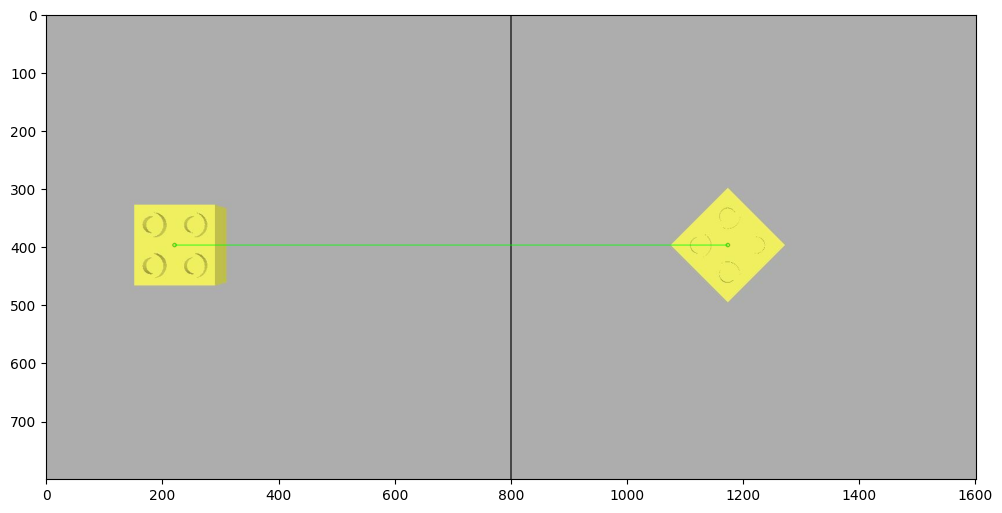
\includegraphics[width=\textwidth]{figures/ideal_centre-of-mass.png}
    \caption{Centre of mass matching}
    \label{fig:centre-of-mass}
\end{figure}

However, note that while a single point is enough to compute the translation offset between the object in different scenes, it is not sufficient to compute the orientation offset. By reducing the object in the image to a single point, we have estimated its position, but have no information about its orientation. This is a problem for us since we want the system to be robust to not only moving the object, but also rotating it. Some objects may behave very differently in different orientations if they do not have rotational symmetry. As such we need a way to estimate the orientation of the object in both images.\\

In order to achieve this we cannot reduce the object to a single central point, but we can reduce it to a collection of points. Having multiple points which match in the two images can allow us to identify if a translation or rotation have occurred. \reffig{fig:ideal-matches} shows how an ideal set of matches allows us to infer both a translation and rotation between the object in the images. In this case we can see the block needs to move to the right of the frame, but now also needs to rotate approximately 45$\degrees$ anticlockwise (a positive rotation according to the right hand rule) about the vertical axis.

\begin{figure}[h]
    \centering
    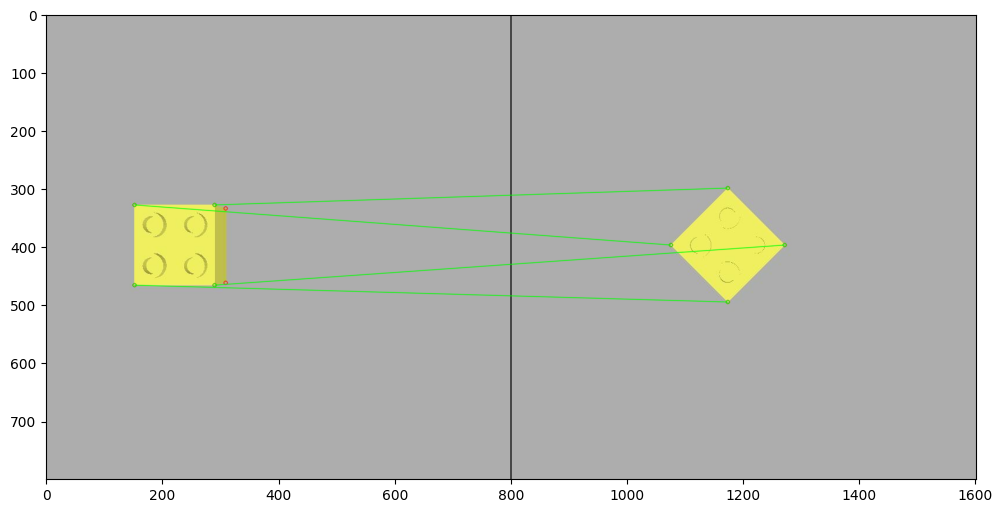
\includegraphics[width=\textwidth]{figures/ideal_matches.png}
    \caption{Ideal keypoint matching}
    \label{fig:ideal-matches}
\end{figure}

Note that this is only one way the keypoints could be matched. \reffig{fig:ideal-matches-inv} shows another way we may choose to match the keypoints. In this case the live object should move to the right and rotate approximately 45$\degrees$ clockwise (a negative rotation according to the right hand rule) about the vertical axis, in order to align with the demonstration object. While having multiple possible ways to match the keypoints may seem like a problem, this is merely a consequence of the object in question having rotational symmetry. It does not matter which way we rotate the object, because it will behave the same, whichever side we are facing, and each side is indistinguishable from each other. As such, for our purposes it would not matter which matching and subsequent transformation we chose, since in either case the object is aligned to the demonstration image. In practice this situation would not likely occur, since we will have many more keypoints, and the keypoints will very likely not be evenly spaced as in this ideal example.

\begin{figure}[h]
    \centering
    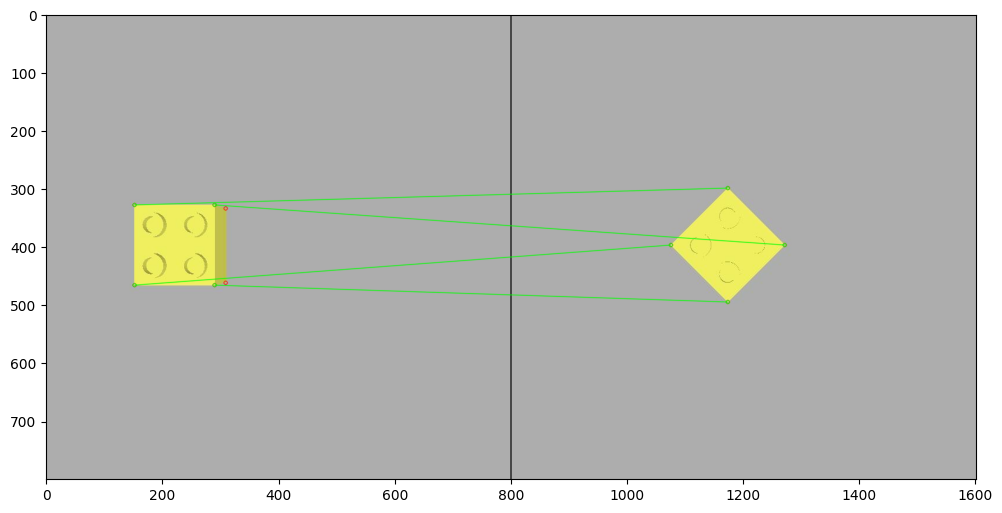
\includegraphics[width=\textwidth]{figures/ideal_matches_inv.png}
    \caption{Alternative ideal keypoint matching}
    \label{fig:ideal-matches-inv}
\end{figure}

We can also see that in both figures, the live image contains two additional keypoints marked in red. These keypoints could not be matched to any in the demonstration image so are ignored when calculating the translation and rotation to align the objects. In this case it is because these keypoints become occluded when we view the object in the demonstration image.\\

These figures are designed to give an intuition for how we can use keypoints to find the desired end effector offset. In these figures we have considered ideal keypoints where the keypoints are extracted on useful points of the image, namely the object corners, and where the matching is perfect with no mistakes. These keypoints have been placed by a human for the purposes of demonstration. Obviously for the complete system we want the keypoint extraction and matching to be automated. How we achieve this will be explored next.

%TODO undecided whether this or kabsch section should come first
\subsection{Automated keypoint extraction and matching}
\label{subsec:keypoint-algos}
Keypoint extraction is a popular and well studied problem in the field of computer vision. As such we have many options at our disposal. Our goal is to identify the pixels where the image changes significantly. These may be where 
%TODO mention experiments in evaluation section which tells us the best algorithm for extraction and matching

\subsection{Calculating end effector offset}
\label{subsec:kabsch}
Now that we have a list of matched keypoint pairs, we can begin to calculate the offset between the object in the live and demonstration image. Fortunately there exists an algorithm for computing the translation, rotation and scaling, which best maps a set of points onto another set of points. This algorithm is called the \socalled{Kabsch-Umeyama algorithm}. The algorithm takes in two sets of points, a reference set P, and a test set Q. It computes a translation t, a rotation matrix R and a scale factor s, such that when these transformations are applied to Q, yielding Q', the root mean squared distance between P and Q' is minimized. For our purposes we make a number of important modifications to the original algorithm to better fit our 

As mentioned above, we decide to convert all keypoints to world coordinates first. By doing this we can more easily include the depth information of the image. Additionally, this will result in the translation computed already being in world coordinate units, meaning no further calculation is needed to calculate how far to move the end effector.\\

...
The first step of the algorithm will look familiar to something we tried in \refsubsec{subsec:keypoints}. The first step is to compute the centroids of the two sets of points. This is just the average position of all the points in the set. This acts like the centre of mass of the point set. With sufficiently many and well spaced keypoints in our set, this centre of mass will be approximately equal to the centre of mass we computed earlier by considering all pixels of the object. As we discussed earlier, the centre of mass of the points will be enough to compute the translation between the two sets.
$$\overline{p} = \frac{1}{|P|}\sum_{p \in P}p \longspace \overline{q} = \frac{1}{|Q|}\sum_{q \in Q}q$$
The next step is to re-centre the points so that the centre of mass is on the origin. It is therefore clear that to achieve this we will 
... covariance shit
After 

%TODO mention experiments for how it behaves with noise applied to ideal matches.
% create random unit vector, and random magnitude of noise. This way we can ensure noise is in a tight window. So we can say this is how it perfromed with 1-5 pixels noise, 5-10. Better than 1-5 and 1-10.


%keypoint extraction - diagrams to show how we extract keypoints, what sort of parts are keypoints due to change in derivative.
%  - SIFT vs BRIEF/ORB
% 
% Keypoint matching - the different distance metrics for SIFT and ORB.
%  diagrams for how matching can help us identify translations and rotations, ideal matches
% GMS (Do more research as to how it works) and how we refine matches into better matches for our purposes
% calculating transformation from matches (not sure where this section should go. Could move higher up to motivate why we extract keypoints at all)
% Go through the equations, cite Kabsch algorithm, explain why we compute translation without R since we consider rotation as spinning in place and so translation is just the offset in centroids.

\newpage




\section{Decomposing the reward function}
\label{sec:reward-function}
At this point we have a system which can transform a trajectory from the demonstration environment to a new unseen environment containing the same object. Our goal now is to extend this system to transform the trajectory into an environment containing different objects. The current system will select the demonstration whose context image matches the current scene most closely. This allows it to select the correct demonstration whose context image contains the target object in the current scene. However, this naturally extends to unseen objects since the similarity metric used will still compare the current scene to all context images and select the most similar. We can expect the similarity between the embeddings of the two images to be greatest when they contain the same objects, however if no such demonstration exists on this specific object, we can still select whichever demonstration is closest. Since we directly compare not the images themselves, but the image embeddings from the vision transformer, this translates to selecting the image with the object whose dino feature points are most similar. In essence, the object which behaves most similarly to the current scene object. Therefore we can expect the system to already choose the demonstration which is closest to working with this new object. For example if the demonstration was to pick up a can, it is likely that when faced with a bottle in the current scene that the system would select the can demonstration. This is because the objects appear similar as they are both cylindrical items, and the robot would have to interact with them in similar ways, by grasping around the cylinder. As such we can conclude that the can demonstration is the closest one to working with this new object.
%TODO check this paragraph isnt too rambly
%also should this be at the start of this section or the end of the prev one?
% I think the prev one

The hope would be that these two objects are similar enough that the same demonstration would already be able to successfully complete the task on this new object.

%TODO the later stuff is no longer relevant but the above paragraph could still be good to talk about. Just slightly reword stuff to sound like this is a happy bonus rather than the original focus


Designing the reward function to score how good an executed trajectory was will be very complicated since we need to encode so many intuitive notions into rigorous mathematics. For example, if the trajectory ends in some state $s$ then we want to ask \speech{Does this state represent some task having been completed?} This is very hard to do since the task could be anything, and we have little prior knowledge of what the robot was intending to achieve. Additionally for each state along the trajectory we would also ask questions of \speech{Is this state interesting?} \speech{Is this state unlike states we have seen before?} \speech{Was this state what we expected to happen by completing these actions, or was the outcome surprising?} We need ways to mathematically encode each of these questions from the series of state, action pairs along the robot's trajectory. We will also need to weight the relative importance between each aspect of the reward function.\\

We start by considering how to categorise the above questions. Particularly we may notice that the question of \speech{Was a task completed?} concerns primarily the final state of the trajectory. It wants to know information external to the trajectory itself, particularly, was a meaningful task accomplished by this trajectory. The other questions however, ask about the inherent properties of the trajectory, were the states involved interesting, novel or surprising? These two different categories are called extrinsic and intrinsic rewards respectively. Our final reward function will be some combination of both types.\\
\textbf{\textit{Extrinsic rewards}} motivate the agent to learn to complete a specific task. The specifics of the trajectory itself are unimportant, if the task has been completed then a high reward is given. The problem with extrinsic rewards is that they are by definition, dependent on the task at hand. This requires us to define a reward function for each task. This flies in direct opposition to the goal of this paper which is to produce an agent which can learn to perform new tasks which were unseen in the demonstrations. One potential solution is to use external rewards. This strategy does not have an analytically defined reward function. Instead we ask a human for input to decide the reward the robot gets for this trajectory. This could be on a scale from 0 to 1 where 1 is perfectly completing the task. This system has promise because despite requiring human input, it offloads the complex intuition required to properly score the trajectory. Specifically because the agent is attempting to solve new tasks, the human is able to infer what the robot was going for, and grade accordingly. If the robot manages to pick up an object, we can be reasonably sure this was the goal of the task, and it has therefore been completed. This high level reasoning about what the task was and subsequently has it been achieved, would be very difficult for a computer system to evaluate.\\
\textbf{\textit{Intrinsic rewards}} in contrast, motivate the agent to produce better trajectories. For example trajectories which are different from other previously seen trajectories. These rewards are concerned only by the internal properties of the trajectories and do not care about the impact this trajectory has on the external environment.




% \chapter{Project Plan}
% \label{chap:plan}


% \section{Technical Progress}
% Technical progress so far has been limited while a focus has been put on research and writing this interim report. The main implementation achievements thus far have been on important utilities for later in the project. In particular downloading the necessary files and initialising the simulator is obviously key to the success of this project and so was completed as a priority.\\

% Following this, a utility program was created for generating demonstration trajectories. As discussed in Chapter \ref{chap:background}, this project aims to use imitation learning to teach the agent an initial collection of skills. As such, a program to streamline the collection of demonstrations for the imitation learning will be a useful asset throughout this project.\\

% This program allows for individual joint control by selecting and moving joints independently. Once the arm is positioned in the correct pose, the user can save the current pose as a key frame of the trajectory. From here they can move the arm again and save the next key frame. If a mistake is made, the user can revert the robot arm to the last saved key frame.\\
% The trajectory is stored as a list of joint poses. Each element of the trajectory is a key frame robot state. The key frame stores the joint angles of the robot's 11 joints (although not all joints are actuated so a small number of these 11 joints are permanently fixed at 0 radians).

% The program is written to interface with a video game controller, so that the user can control joint angles using an analogue input method such as the joysticks. This makes the program slightly more user friendly, as moving the joystick only slightly will move the joint very slowly and so allows for finer control.\\
% In addition to controlling joint poses, the program allows for camera rotation and zooming to better see the full robot pose, and colour codes the current joint the user is controlling in the wire-frame view, visible in Figure \ref{fig:arm-wire}.



% \section{Future Plans}
% The project plan can be broken into small short term goals which will be built upon, and longer term goals which constitute the bulk of the project. This project aims to complete the goals by the deadline shown:

% \subsection*{End of January 2024}
% Since very little time remains before the end of January, a very small goal of further improvements to the trajectory generating utility program is set. The program should be modified to allow for a second control mode. Instead of individually controlling each joint angle, it should be possible to control the 3D position of the end effector, and use inverse kinematics to calculate the joint angles from this position. The two control modes should work with each other and be able to switch between them while using the program.

% \subsection*{End of February 2024}
% By the end of February the first stage of the learning algorithm should be in place. This is implementing the one-shot imitation learning algorithm as described by  N. Di Palo, and
% E. Johns \cite{one-shot-imitation}. This first part of the algorithm will allow us to provide the agent with an initial set of skills, from which it can explore and learn more.

% \subsection*{End of March 2024}
% By the end of March this project hopes to implement the next step of the algorithm which involves the noise based exploration of the nearby state space. The agent will select a known skill trajectory and try adding noise to it to investigate what happens. The idea being that the agent selects the most similar skill from its repertoire, and so small amounts of learned noise will be sufficient for a task that nearly succeeded. For example, starting with the trajectory to pick up a water bottle, the agent may be able to learn how to pick up a can by simply augmenting the known trajectory. The action of picking up both objects are very similar, but the robot may need to grab lower on the can since it is shorter than the bottle. This slight deviation will be captured by the noise. Once an amount of noise is learned which is successful at completing the new task, the original trajectory and noise can be saved together as a new skill.\\
% This is a large part of the algorithm and March also contains end of term exams, reducing the amount of time available for the project in the final weeks of March. As such this is a soft deadline, and we anticipate the need for this implementation point to bleed into the next month's milestones.

% \subsection*{End of April 2024}
% By the end of April this project aims to be at the final implementation step. This will include the \socalled{curiosity based reward function} to encourage exploration of interesting or uncertain parts of the state space, which will hopefully lead to more unique and successful skills being learned.\\
% The other feature we plan to implement by April is the human based skill descriptor system. As discussed in Chapter \ref{chap:introduction}, this would allow the robot to demonstrate its self-taught skills where the human can provide context and a name to this skill. This can then be used in a deployed setting with a language model to give the agent orders to complete tasks based on its learned skills.

% \subsection*{End of May 2024}
% The month of May is intended to be used to run larger scale experiments and fine tune the algorithm. By this point the bulk of the implementation should be complete and this project should be looking to collect lots of results, and potentially deploy the agent to a physical robot arm. The transition from simulation to real world will undoubtedly bring challenges through the inaccuracies of real life such as joint frictions or differences in the simulated and true masses of objects and the robot arm segments. These small inaccuracies of the simulation may lead to compounding problems which affect the success rate of the agent. If this is the case then further tuning will be considered to improve the agent again.

% \subsection*{17th June 2024}
% The month of June is reserved for finishing and polishing the final report. By this deadline the project, experiments and accompanying report should all be completed.